\documentclass{article}
\usepackage[T1]{fontenc}
\usepackage{siunitx}
\usepackage{titrages}
\pgfplotsset{compat=1.18}
\titragedefinir{acetique}{
  volume = 10,
  becher = { espece = { pKa = 4.76, C = 0.1, lambda = {0, 4.09} } },
  burette = { base forte = 0.1 },
  volume max = 20,
}
\titragedefinir{phosphorique}{
  volume = 10,
  becher = { espece = { pKa = {7.20, 2.15, 12.35}, C = 0.1 } },
  burette = { base forte = 0.1 },
}
\titragedefinir{ammoniac}{
  volume = 10,
  becher = { espece = { pKa = 9.25, C = 0.1, forme = 1, charge = 1, lambda = {7.35, 0} } },
  burette = { acide fort = 0.1 },
  abscisse = n,
}
\titragedefinir{fort}{
  volume = 100,
  becher = { acide fort = 0.01 },
  burette = { base forte = 0.1 },
  volume max = 20,
  conductivite corrigee = true,
}
\titragedefinir{fortmS}{
  volume = 100,
  becher = { acide fort = 0.01 },
  burette = { base forte = 0.1 },
  volume max = 20,
  conductivite corrigee = true,
  unite = mS/cm,
}
\titragedefinir{melange}{
  volume = 20,
  becher = { acide fort = 0.05, espece = { pKa = 4.76, C = 0.05 } },
  burette = { espece = { pKa = 9.25, C = 0.1, forme = 1 } },
  volume max = 30,
}
\titrageredoxdefinir{cerium}{
  volume = 10,
  becher = { espece = { E0 = 0.77, C = 0.1, forme = red } },
  burette = { espece = { E0 = 1.72, C = 0.1, forme = ox } },
  reference = ECS,
  volume max = 20,
}
\titrageredoxdefinir{dichromate}{
  volume = 10,
  becher = { espece = { E0 = 0.77, C = 0.1 } },
  burette = { espece = { E0 = 1.33, n = 6, H = 14, stoechiometrie = {1, 2}, C = 1/60, forme = ox } },
  pH = 0,
  volume max = 20,
}
\titrageredoxdefinir{vanadium}{
  volume = 10,
  becher = { espece = { E0 = {-0.26, 0.34, 1.00}, n = {1, 1, 1}, H = {0, 2, 2}, C = 0.1 } },
  burette = { espece = { E0 = 1.51, n = 5, H = 8, C = 0.02, forme = ox } },
  pH = 0,
  volume max = 40,
}
\begin{document}
pH initial \titragepHinitial{acetique}, demi-équivalence \titragepH{acetique}{5},
équivalence \titragepH{acetique}{10}, volume à pH 7 : \num{\titragevolume{acetique}{7}}.

Conductivité : \titrageconductivite{acetique}{2} et \titrageconductivite{acetique}{15} S/m ;
fort, corrigée : \titrageconductivite{fort}{10} S/m, soit \titrageconductivite{fortmS}{10} mS/cm.

Rédox : E(5) = \titrageE{cerium}{5}, E(10) = \titrageE{cerium}{10} V/ECS ;
dichromate E(10) = \titrageE{dichromate}{10} ; vanadium : équivalences
\titrageequivalence{vanadium}{1}, \titrageequivalence{vanadium}{2}, \titrageequivalence{vanadium}{3} ;
saut 2 à \titragesaut{vanadium}{2}, E \titragesaut[E]{vanadium}{2} ; volume à 1 V/ECS :
\titragevolume{cerium}{1} ; tangentes depuis 7 mL : \titragetangentes{cerium}{7} mL,
\titragetangentes[E]{cerium}{7} V/ECS.

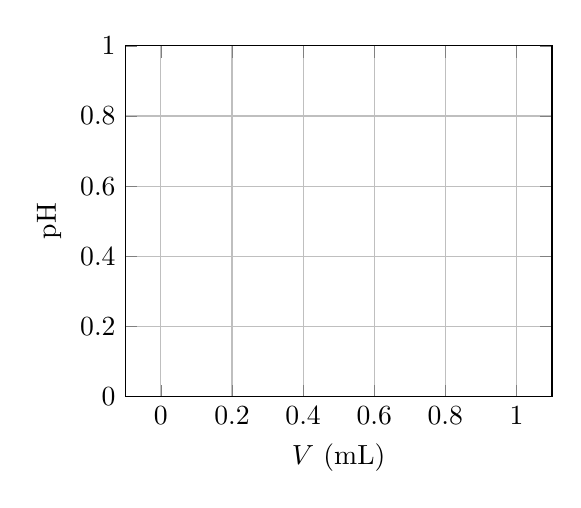
\begin{tikzpicture}
\begin{axis}[xlabel={$V$ (mL)}, ylabel=pH, ymin=0, ymax=14, grid=both, width=7cm]
  \addplottitrage[thick]{acetique}
  \addplottitrage[thick]{phosphorique}
  \addplottitrage[thick]{melange}
  \addplottitragesauts[black, mark=*]{phosphorique}
  \addplottitragetangentes[orange, dashed]{acetique}{7}
\end{axis}
\end{tikzpicture}
\begin{tikzpicture}
\begin{axis}[xlabel={$n$}, ylabel=pH, width=7cm]
  \addplottitrage{ammoniac}
\end{axis}
\end{tikzpicture}

\begin{tikzpicture}
\begin{axis}[xlabel={$V$ (mL)}, ylabel={$\sigma$ (S/m)}, width=7cm]
  \addplottitrageconductivite[thick]{acetique}
  \addplottitrageconductivite[thick]{fort}
  \addplottitrageconductivite[thick]{ammoniac}
\end{axis}
\end{tikzpicture}
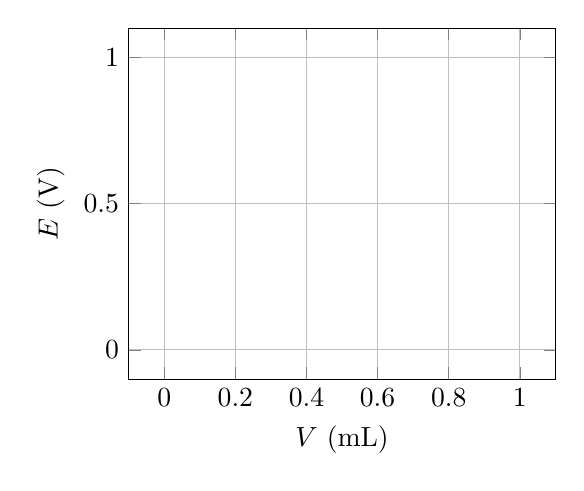
\begin{tikzpicture}
\begin{axis}[xlabel={$V$ (mL)}, ylabel={$E$ (V)}, width=7cm, grid=both]
  \addplottitrage[thick]{cerium}
  \addplottitrage[thick]{dichromate}
  \addplottitrage[thick]{vanadium}
  \addplottitragesauts[black, mark=*]{vanadium}
  \addplottitragetangentes[orange, dashed]{cerium}{7}
\end{axis}
\end{tikzpicture}

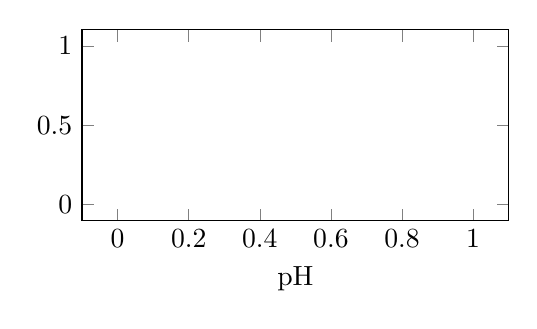
\begin{tikzpicture}
\begin{axis}[xlabel=pH, width=7cm, height=4cm]
  \addplotfractions[thick]{6.35, 10.33}
\end{axis}
\end{tikzpicture}
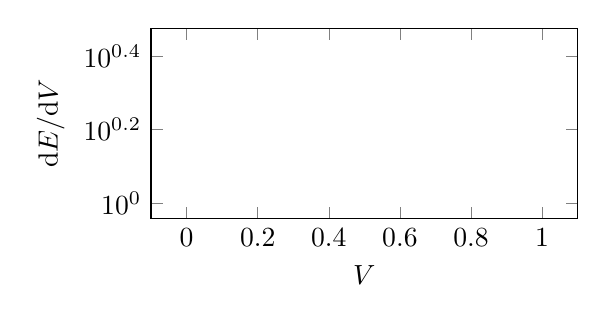
\begin{tikzpicture}
\begin{axis}[xlabel={$V$}, ylabel={$\mathrm{d}E/\mathrm{d}V$}, width=7cm, height=4cm, ymode=log]
  \addplottitragederivee{cerium}
\end{axis}
\end{tikzpicture}
\end{document}
